\documentclass{article}
\usepackage{amsmath}
\usepackage{graphicx}
\usepackage[utf8]{inputenc}
\usepackage[T1, T2A]{fontenc}
\usepackage[english,russian]{babel}

\title{Откуда берутся асимптотические разложения}
\author{Anikin Evgeny, 128}

\begin{document}
\maketitle
Поставим задачу как-нибудь вычислить интеграл 
$$
	J(\alpha) = \int_{0}^{+\infty} \frac{e^{-\alpha x}\,dx}{1 + x} 
$$

\section{Большие $\alpha$}
Пусть $\alpha$ велико: тогда основной вклад в интеграл даёт область около нуля, где
$1/(1+x)$ можно разложить в ряд.

Проделаем такие формальные действия:
\begin{multline}
	J(\alpha) = \int_{0}^{+\infty} \frac{e^{-\alpha x}\,dx}{1 + x} = 
		\int_{0}^{+\infty} dx\,e^{-\alpha x}\sum_{n=0}^{\infty} (-1)^n x^n = \\
		=\sum_{n=0}^{\infty}(-1)^n \int_{0}^{+\infty} x^n e^{-\alpha x} \,dx
\end{multline} 
Вычисляя интегралы под суммой, получим
$$
	J(\alpha)=\int_{0}^{+\infty} \frac{e^{-\alpha x}\,dx}{1 + x}  = 
		\sum_{n=0}^{\infty}\frac{(-1)^n n!}{\alpha^{n+1}}
$$
Полученный ряд расходится. Тем не менее, его можно использовать для приближённого 
вычисления интеграла.

На рисунке видно, что разложение до высоких порядков имеет смысл только для больших $x$.
При малых $x$ справедливы только низшие порядки.

\begin{figure}[h]
	\centering
	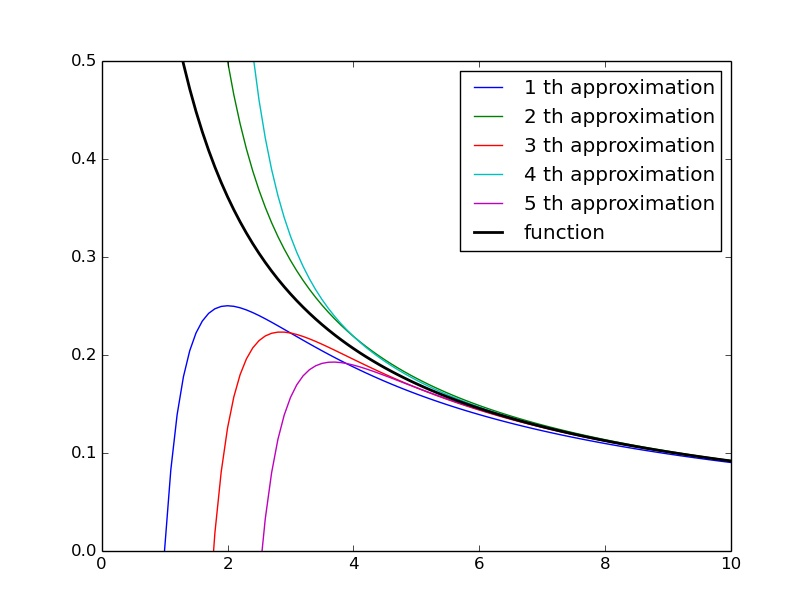
\includegraphics[width=0.9\linewidth]{expansion.jpeg}
	\caption{
		На рисунке изображены графики частичных сумм ряда (цветные) и исходного интеграла
		(чёрный)
		}
\end{figure}

\section{Малые $\alpha$}
Проделаем следующие преобразования:
\begin{multline}
	J(\alpha) = \int_{0}^{+\infty} \frac{e^{-\alpha x}\,dx}{1 + x} = 
	 	\int_{0}^{+\infty} \frac{e^{-x}\,dx}{\alpha + x} = \\
		=e^{\alpha} \int_{\alpha}^{\infty} \frac{e^{-x}\,dx}{x}  
		=e^{\alpha}\left( \int_{\alpha}^{1} \frac{e^{-x}\,dx}{x}+ 
			\int_{1}^{\infty} \frac{e^{-x}\,dx}{x} \right) = \\
		=e^{\alpha}\left( \log{\frac{1}{\alpha}} + \int_{0}^{1}\frac{e^{-x} - 1}{x}\,dx + 
			\int_{1}^{\infty} \frac{e^{-x}}{x}\,dx
			-\int_{0}^{\alpha} \frac{e^{-x} - 1}{x}\,dx \right)
\end{multline}
Два интеграла в середине --- константы, а последний интеграл может быть вычислен
разложением подынтегральной функции в ряд Тейлора. Таким образом мы получим
разложение $J(\alpha)$ в ряд Тейлора (не считая логарифмического члена).
\end{document}
